\documentclass[11pt]{beamer}
\usetheme[
  workplace=fi,
]{MU}

\usepackage{hyperref}
\usepackage[utf8]{inputenc}
\usepackage[english]{babel}
\usepackage[T1]{fontenc}
\usepackage{amsmath}
\usepackage{amsfonts}
\usepackage{amssymb}
\usepackage{graphicx}
\usepackage{listings}
\usepackage{pgf}
\usepackage{tikz}

\usetikzlibrary{arrows,automata,positioning}

\author{Jan Tušil}
\title{Formal Semantics of C++ language? Why?}
%\setbeamercovered{transparent} 
%\setbeamertemplate{navigation symbols}{} 
%\logo{} 
\institute{FI MU} 
\date{11.4.2018} 
%\subject{}


\lstset {
	basicstyle=\ttfamily
}

\newcommand{\backupbegin}{
   \newcounter{finalframe}
   \setcounter{finalframe}{\value{framenumber}}
}
\newcommand{\backupend}{
   \setcounter{framenumber}{\value{finalframe}}
}


\begin{document}

%%%%%%%%%%%%%%%%%%%%%%%%%%%%%%%%%%%%%%%%%%%%%%%%%%%%%%

% Phase 1: Attention
% If I go first:
% Good morning everyone. It is a pleasant surprise that there are
% so many of us in such an early hour. Did you sleep well?
% I hope you did, so you will not fall asleap now.
% If I go second:
% Good morning everyone. I hope you are enjoing the presentations
% as much as I do. Now you are hopefuly woke up enough not to fall asleap
% during my talk. The talk is about the project of
% defining formal semantics of C++.

\begin{frame}
\titlepage
\end{frame}


% Phase 3: Credibility (20s)
% As I have said, my name is Honza Tusil
% and I am currently a Ph.D. candidate at FI MU.
% My research interested include software verification,
% programming language semantics and programming languages
% in general. I am also tutoring some C and C++ related classes
% and in past I did some part-time C/C++ development on embedded systems for a local company.
\begin{frame}{About me}
\begin{columns}

\begin{column}{0.30\textwidth}
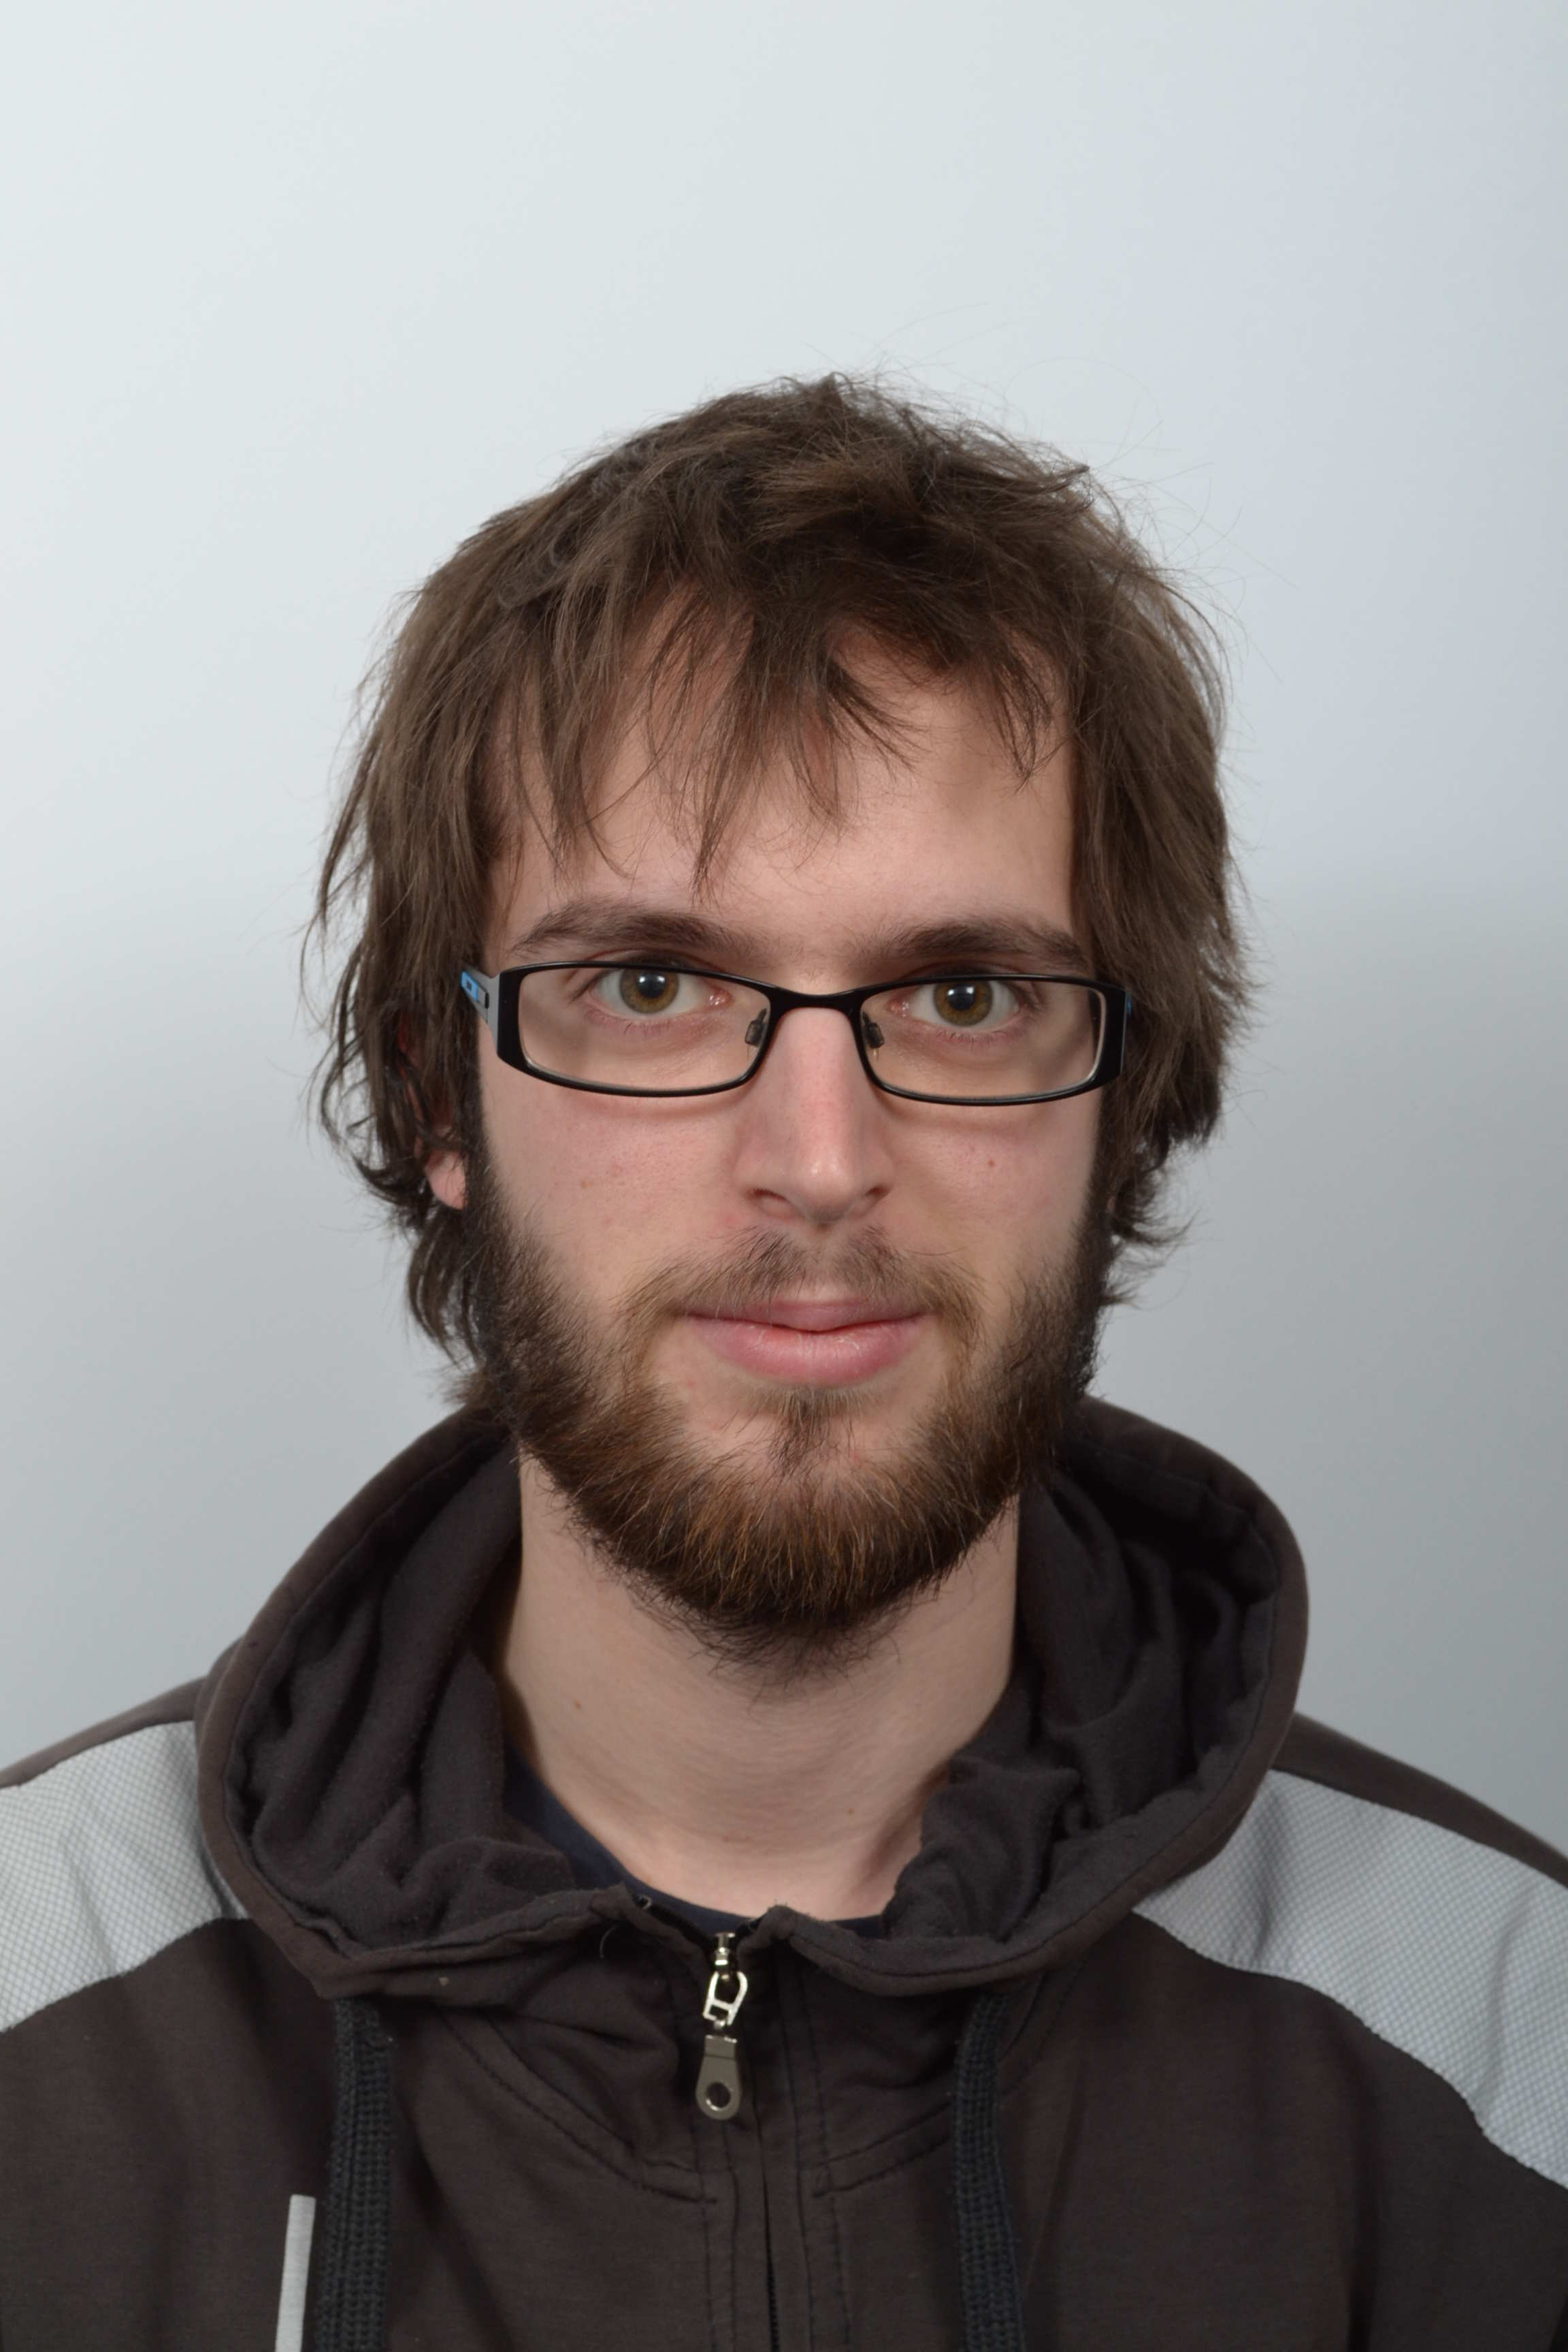
\includegraphics[width=1.0\linewidth]{img/me.jpg}
\end{column}
\begin{column}{0.7\textwidth}
\begin{itemize}
\pause \item research: SW verification, PL semantics
\pause \item teaching: programming in C (PB071) and C++ (PB161)
\pause \item past: C/C++ @ embedded systems (local company)
\pause \item \url{jan.tusil@mail.muni.cz}
\pause \item \url{https://www.fi.muni.cz/~xtusil/}
\end{itemize}
\end{column}
\end{columns}
\end{frame}

% In the following ten minutes I would like to talk about the following. First I am going to show the current situation 
% of C++ analysis/verification tooling, then I will explain how
% is my Master thesis to this, and finally I am going to
% show the future work I would like to do.

\begin{frame}{The Structure}
\tableofcontents
\end{frame}

\AtBeginSection[]
{
  \begin{frame}
    \frametitle{The Structure}
    \tableofcontents[currentsection]
  \end{frame}
}

\section{The Context}
%\section{Why bother?}

% Modern programming languages are really powerful - but also
% really complex. The specification of the C++ language alone
% has circa 380 pages, and the language and its standard library
% together has 1400 pages in total.
% As the time goes, some features are being added to the language,
% other are being removed. For the C++ language there is
% a nice map of the features. It looks like this.
%\begin{frame}{The C++ lands}
%\pause
%\includegraphics[trim=100 900 1700 300, clip, width=1.0\linewidth]{img/cppmap.png}
%\end{frame}
    
{
  \usebackgroundtemplate{\includegraphics[trim=100 900 1700 300, clip, height=\paperheight,width=\paperwidth]{img/cppmap.png}}
  \setbeamertemplate{navigation symbols}{}
  \begin{frame}[plain]
  \end{frame}
}

% And this is the full map
\begin{frame}{The C++ lands}
\includegraphics[width=0.9\linewidth]{img/cppmap.png}
\end{frame}


% 2 min


% The C++ language is complex and we
% - the programmers - make mistakes.
% Therefore we have a plenty of tools which help as to find
% bugs in our programs, or to prove their absence from the code.
% The last two tools in the list are being actively developed
% here on Faculty on Informatics.

% The tools can give programmers a valuable information.
% For example, that their program contains an error.
% Or that some code is suspicious, and it could be an error.
% Or they can say that the program is error-free.
\begin{frame}{The complexity of C/C++}
\begin{columns}

\begin{column}{0.5\textwidth}
Some of the tools:
\begin{itemize}
\pause \item clang-tidy
\pause \item frama-c
\pause \item cbmc
\pause \item divine
\pause \item symbiotic
\end{itemize}
\end{column}

\begin{column}{0.5\textwidth}
\pause
Possible outputs:
\begin{itemize}
\pause \item error
\pause \item suspicious code, possible error
\pause \item correct
\pause \item unknown
\end{itemize}
\end{column}

\end{columns}
\end{frame}

% This, however, leads to some important questions.
% Are they correctly implemented?
% Do these tools understand the C++ language correctly?

% There exists a competetion of verification tools, called SV-COMP.
% In this competetion, two set of C programs are used:
% a set of correct programs, and a set of incorrect programs.
% However, two years ago it was discovered that some of the programs
% in the 'correct' set are actually incorrect (they contain
% an undefined behaviour). So the tools that classify such programs
% as correct gain some points in the competetion, but actually
% they contain an error - they do not understand the C language
% correctly.
\begin{frame}{Some disturbing questions}

\begin{itemize}
\pause \item Are they correctly implemented?
\pause \item Do they really ,,understand'' C++?
\pause \item SV-COMP: programs containing undefined behavior in the set of correct ones\footnote[frame]{\uncover<4->{https://runtimeverification.com/blog/?p=200}}
\end{itemize}

\end{frame}


% One possible solution to this problem is to use
% a translator from the desired language to some simpler language.
% A natural choice is to use a compiler. Many tools,
% including Divine, Klee, and Symbiotic,
% use a compiler called 'Clang' to translate the source code
% to a program in so-called LLVM Intermediate Representation.
%
% TODO: an image
\begin{frame}{Solution no. 1 - use a compiler}
%Use a translator from the desired language to some simpler language.

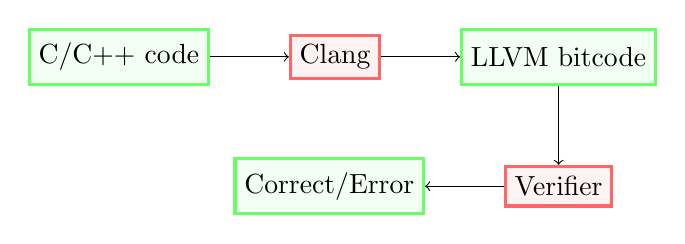
\begin{tikzpicture}[
%data/.style={circle, draw=green!60, fill=green!5, very thick, minimum size=7mm},
data/.style={rectangle, draw=green!60, fill=green!5, very thick, minimum size=7mm},
tool/.style={rectangle, draw=red!60, fill=red!5, very thick, minimum size=5mm},
]
%Nodes
\node[data]        (source)                           {C/C++ code};
\node[tool]      (compiler)     [right=of source]   {Clang};
\node[data]        (bitcode)      [right=of compiler] {LLVM bitcode};
\node[tool]      (verifier)     [below=of bitcode]  {Verifier};
\node[data]        (answer)       [left=of verifier]  {Correct/Error};
 
%Lines
\draw[->] (source.east) -- (compiler.west);
\draw[->] (compiler.east) -- (bitcode.west);
\draw[->] (bitcode.south) -- (verifier.north);
\draw[->] (verifier.west) -- (answer.east);
\end{tikzpicture}

%E.g. a compiler (clang/llvm). This way the tool does not have to understand the complex C++ language, because the compiler understands it.

\end{frame}


% I can see two disadvantages of this approach. First,
% it is not clear how to verify the correctness with respect to the programming language,
% because during the translation, some undefined behavior may become defined.
% And second - on the level of simpler language we might not be able to express
% some higher-level properties of the program. And therefore we are not able to prove
% or disprove them.
\begin{frame}[fragile]{Limitations}
\begin{columns}

\begin{column}{0.45\textwidth}
\pause
An undefined behavior may become defined.
\pause
\begin{lstlisting}
int x = INT_MAX;
x++;
\end{lstlisting}
\end{column}

\begin{column}{0.55\textwidth}
\pause
Template-based polymorphic code.
\pause
\begin{lstlisting}
template <typename It>
void sort(It begin, It end);
\end{lstlisting}
\end{column}

\end{columns}
\end{frame}


% A different approach is to have an executable formal semantics
% of given language, and derive everything else from that.
% This is implemented in a framework called "K".
% In the framework, one can define tools and languages independently,
% and then instantiate any desired tool with a desired language.
% The set of tools may include a parser, an interpreter,
% a compiler, a model checker, test case generator,
% a symbolic executor...
% Some of them are already programmed.
\begin{frame}{Solution no. 2 - have a formal semantics}

\begin{center}

\pause
$$ \left( W, R \right) \textbf{ where } W = \left( \textsc{Program}, \textsc{Store} \right) \textbf{ and } R \subseteq W \times W $$

\pause
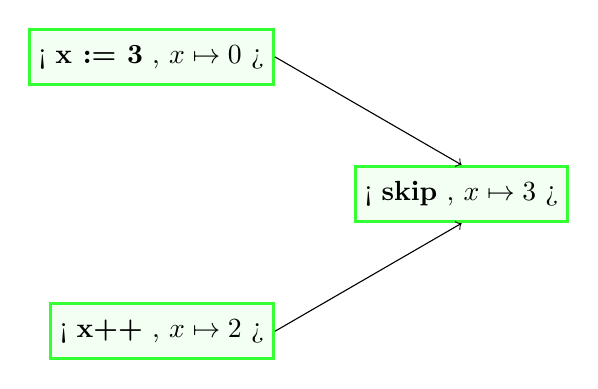
\begin{tikzpicture}[
%data/.style={circle, draw=green!60, fill=green!5, very thick, minimum size=7mm},
state/.style={rectangle, draw=green!80, fill=green!5, very thick, minimum size=7mm},
]
%Nodes
\node[state]   (st2)                           { < \textbf{skip} , $x \mapsto 3$ > };
\node[state]   (st0)      [above left=of st2]  { < \textbf{x := 3} , $x \mapsto 0$ > };
\node[state]   (st1)      [below left=of st2]  { < \textbf{x++} , $x \mapsto 2$ > };
 
%Lines
\draw[->] (st0.east) -- (st2.north);
\draw[->] (st1.east) -- (st2.south);
\end{tikzpicture}

\end{center}

\end{frame}

\begin{frame}{K Framework}
\begin{center}
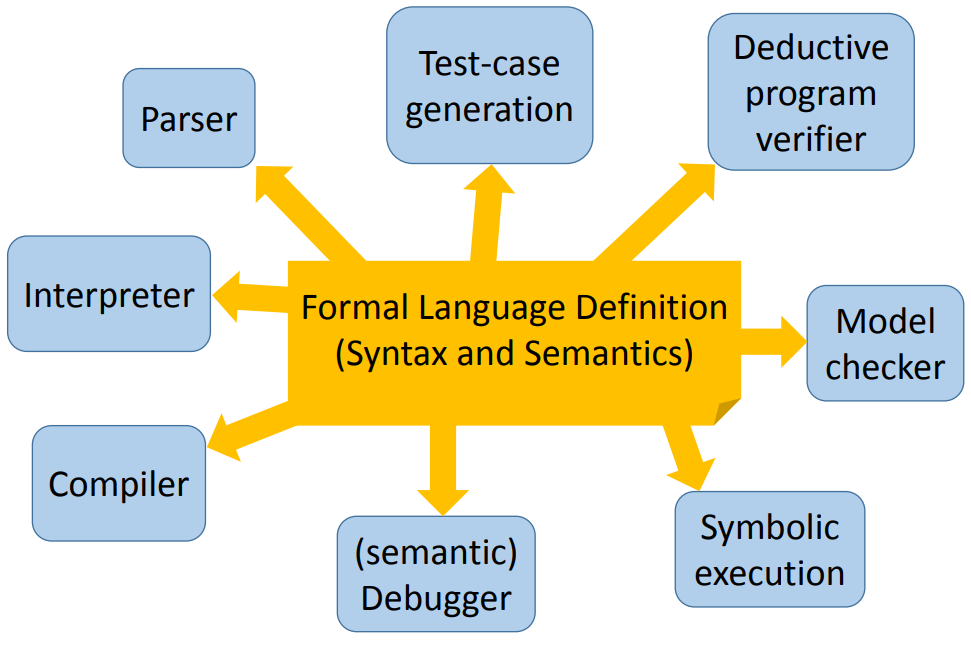
\includegraphics[width=0.7\linewidth]{img/kidea.png}
\end{center}
\end{frame}

% Several laanguages were already formalized in K, including Python,
% JavaScript and C. The semantics of C was used to build a commercial
% tool RV-Match for discovering of undefined behavior.
% Nowadays the semantics is being extended with the support of C++.
\begin{frame}{C/C++ @ K}
\begin{itemize}
\item Already formalized: Python, JavaScript, C
\pause \item Application of the C semantics: RV-Match \\

\includegraphics[width=0.3\linewidth]{img/rvmatch.png}
\pause \item current work: extend the C semantics to C++
\end{itemize}
\end{frame}

\section{Ms Thesis}

% In my MS Thesis I worked on parts of the formal C++ semantics.
% My results are:
\begin{frame}{My Ms Thesis}
Implemented:
\begin{itemize}
\pause \item enumerations
\pause \item zero initialization of class types
\pause \item compile-time function evaluation (a proof of concept)
\end{itemize}
\pause
Found bugs in:
\begin{itemize}
\pause \item GCC (1 bug)
\pause \item CLang (1 bug)
\pause \item The C++ standard (1 defect)
\end{itemize}
\end{frame}


% This is how enums look in C++11
\begin{frame}[fragile]{C++11 \texttt{enum}s}
\begin{lstlisting}[language=C++]
enum E0 { A = 5, B = A + 3 };
enum E1 : char;
enum class E2 : unsigned int;
enum class E3;
enum E5 { A, B } __attribute__((packed));
std::underlying_type_t<E5> x = 5;
\end{lstlisting}
\end{frame}

% In C++, some classes of functions can be evaluated in compile time.
% As the standard evolves, there are less and less restrictions.
% Recursion, cycles in code is not a problem.
% The result of a function evaluated in compile time
% can be used anywhere a compile-time constant is needed.
\begin{frame}[fragile]{Compile time function evaluation}
\begin{lstlisting}
constexpr int fact(int n) {
	return n <= 1 ? 1 : n * fact(n - 1);
}
int main() {
	constexpr int f_4 = fact(4);
	enum class Facts {
		F_4 = f_4,
		F_5 = fact(5)
	};
	assert(int(Facts::F_4) == 24);
	assert(int(Facts::F_5) == 120);
}
\end{lstlisting}
\end{frame}


% Přestože jsem to původně neměl v úmyslu, na popud jednoho z hlavních vývojářů projektu
% jsem implementoval vlastnost, která se nazývá "nulová inializace tříd".
% Myslel jsem si, že to bude hračka, ale zabralo mi to dost dlouhou dobu.
% Jedním z důvodů byla i chyba v projektu, která se projevovala až tehdy,
% když jsem se pokoušel nulovou inicializaci naimplementovat. Chybou byl
% nedeterminismus v sémantice, který umožňoval interpretovat některé programy vícero způsoby.

% There is one rather technical thing I implemented.
% It is a rather tricky thing, but, roughly speaking,
% the point is that when initializing a variable of a class type,
% under some cicrumstances its members get initialized to zero.
\begin{frame}[fragile]{Zero initialization of class types}
\begin{lstlisting}
struct S {
	virtual ~S() = default;
	int x;
};

S s1;
S s2{};
assert(s1.x == 0); // ok
assert(s2.x == 0); // fail
\end{lstlisting}
\end{frame}

%% Tím se dostáváme k poslednímu bodu - opravě některých stávajících chyb.
%
%% Projekt C++ sémantiky v K je stále v experimentální fázi,
%% a tak se při práci častokrát stalo, že jsem narázil
%% na nějakou chybu či nedokončenou implementaci. Opravoval jsem zejména
%% ty, které mi nějak překážely.
%
%% Ještě doplním, že z těchto čtyř bodů byly jen první dva
%% součástí mého oficiální zadání.
%\begin{frame}{Oprava stávajících chyb v projektu}
%
\includegraphics[width=0.5\linewidth]{img/bug.jpg}
%\end{frame}


\section{Future work}

% So what now?
% There are still a few things
% which need to be merged into upstream.
% The support for compile time function evaluation
% needs to be finished, and also many other C++ features.
% On this I am cooperating with a company RuntimeVerification inc.
\begin{frame}{Future of the semantics}
\begin{itemize}
\pause \item Merge the rest to upstream.
\pause \item Finalize \texttt{constexpr}.
\pause \item Templates, threads, bit fields, fold expressions, \ldots
\pause \item How to deal with language changes (C++14, 17, 20, \ldots) ?
\pause \item A cooperation with RuntimeVerification inc.
\end{itemize}
\end{frame}


% Kromě toho bych rád implementoval podporu kontraktů a jejich verifikace
% (jak statické, tak dynamické). Verifikace kontraktů
% u programů s vysokou úrovní abstrakce je vlastně ten důvod,
% kvůli kterému jsem na sémantice jazyka C++ začal pracovat.

% TODO maybe: correctness of an implementation of an analysis

% Rád bych tedy ve zbývajících dvou minutách ukázal,
% jak si takové kontrakty představuji. Na slajdu vidíme
% deklaraci šablonové funkce sort(), která bere dva iterátory
% libovolného typu a seřadí rozsah jimi zadaný.
% Tato funkce požaduje, aby iterátory tvořily platný rozsah,
% tedy aby bylo možné doiterovat od prvního ke druhému.
% Funkce garantuje, že po jejím dokončení bude tento rozsah seřazený.
% Jméno is_sorted v kontraktu této funkce je název úplně obyčejné
% šablonované funkce v jazyce C++, která zkontroluje,
% že rozsah jí předaný je seřazený.
%
% Kontrakty by tedy měly umět pracovat s běžnými výrazovými
% prostředky jazyka C++, zejména s šablonami, funkcemi,
% iterátory a jinými uživatelsky definovanými abstrakcemi.
% Jak na to - uvidíme.

% One thing I would like to do in future
% is verification of generic code which uses template polymorphism.
% For example, there is a generic function 'sort',
% which can be given a range of an arbitrary type,
% and it sorts the range. The behaviour of this function
% is specified with use of Contracts, which is a feature
% which will probably be standardized in C++20.
% Here the function expects that the given pair of iterators
% form a range, and it ensures that when it finishes,
% the range is sorted. One interesting thing here
% is that the contract can be given in terms of
% ordinary C++ functions - in this case, 'valid_range' and 'is_sorted'.
% Even more interesting thing is that valid_range does not return a bool,
% but just 'void' - a type with only one value.
% One mor thing: when the function valid_range is undefined
% on a given input, it means that the expectation of 'sort'
% is not met, so it does not have to sort the range.
\begin{frame}[fragile=singleslide]{Contracts on generics (C++ templates)}
\begin{lstlisting}
template <typename It>
bool is_sorted(It begin, It end);

template <typename It>
void valid_range(It begin, It end);

template <typename It>
void sort(It begin, It end)
  [[ expects axiom: valid_range(begin, end) ]]
  [[ ensures: is_sorted(begin, end) ]] ;
\end{lstlisting}
\pause This is the actual syntax proposed for C++20.
\end{frame}


\begin{frame}{Contracts}
\begin{itemize}
\pause \item What do they mean?
\pause \item Can we evaluate effectful functions in pre/postcondition?
\pause \item How to verify them?
\pause \item How to use existing abstractions and patterns?
\pause \item Can we use the Concepts from C++20?
\end{itemize}
\end{frame}

\begin{frame}{Sources}
\begin{itemize}

\item The C++ map \url{https://fearlesscoder.blogspot.cz/2017/02/the-c17-lands.html}
The diagram of K \url{http://fsl.cs.illinois.edu/index.php/From\_Rewriting\_Logic,\_to\_Programming\_Language\_Semantics,\_to\_Program\_Verification} \\

\item RV-Match \url{https://runtimeverification.com/match/}

%\item Brouk \url{http://cliparting.com/free-bug-clipart-30526/}

\end{itemize}
\end{frame}

\backupbegin

\section{A Bonus for C++ Folks}


% Tohle bych mohl mozna presunout do bonusu.
% Tady bych jenom dodal, že nalezení chyb v překladačíh
% nebo standardech programovacích jazyků není až tak moc neobvyklé,
% zvlášť v kontextu formalizace těchto jazyků - JavaScript, Ethereum.
%\subsection{Chyby nalezené v jiných projektech}

% Během práce jsem hodně pracoval se standardem jazyka C++,
% a když jsem o C++ zjišťoval nové věci, prakticky jsem je zkoušel
% na malých příkladech. Kladl jsem si otázku, "co se stane, když..."?
% Tímto způsobem jsem našel chybu v překladači GCC.
% Kód na slajdu je platný C++ kód, a Clang nebo MSVC jej bez problémů zkompilují,
% nicméně GCC jej odmítne zparsovat. Chybu jsem nahlásil do bugzilly projektu
% a jeden z hlavních vývojářů ji potvrdil.
\begin{frame}[fragile=singleslide]{The bug in GCC}
\begin{lstlisting}
enum E : int;
enum ::E : int{};
\end{lstlisting}
\end{frame}

% Další chybu jsem objevil v překladači clang.
% Chyba se týká toho, v jakém scope žijí konstanty výčtového typu
% (v našem případě konstanty A a B).
%
% Podle jednoho z vývojářů překladače clang, konkrétně správce
% C++ frontendu tohoto překladače, se příčina této chyby projevuje
% i v jiných případech, ve kterých nemá vliv na korektnost, ale jen
% na výkon překladače.
\begin{frame}[fragile=singleslide]{The bug in Clang}
\begin{lstlisting}
namespace N { enum E : int; }
enum N::E : int {A,B};
namespace N {
    int x = int(::N::B); // 1
}
int y = int(::A); // 2
int z = int(A); // 3
\end{lstlisting}
\end{frame}

\begin{frame}[fragile=singleslide]{The bug in C++ standard}
\begin{lstlisting}
enum class E {
    A,
    B = E::A // 1
};
\end{lstlisting}
What is the type of \lstinline|E::A| in (1)?
\end{frame}

\backupend

\end{document}